\chapter{Theoretical Background}
\label{ch:basics}
This chapter introduces the fundamental concepts and theories used in transportation network analysis. We begin with basic graph theory definitions essential for understanding networks. Next, we explore graph construction methods and the importance of sparsity in representing transportation systems as graphs. We then examine clustering algorithms applied to identify communities within these networks, highlighting techniques particularly suited for transportation systems. Finally, we discuss shortest path algorithms that enable efficient route determination between locations in the network.
\section{Basic Definitions}
\label{se:BasicDefinitions}

A graph $G$ is formally defined as an ordered pair $G = (V, E, W)$ comprising a set $V$ of vertices or nodes and a set $E$ of edges, which are 2-element subsets of $V$ . The fundamental components of a graph include: \textbf{Vertices (Nodes)} which represent distinct entities in the network; \textbf{Edges} which represent the connections or relationships between vertices; \textbf{Affinity Matrix} $W$, which is a square matrix where each element $W_{ij}$ represents the weight between vertices $i$ and $j$, indicating distances, travel times, costs, or other metrics.


\section{Graph Construction Methods and Sparsity}
\label{se:GraphConstructionMethodsAndSparsity}

Graph construction methods determine how nodes in a network are connected, playing a crucial role in creating accurate transportation network representations by balancing connectivity with computational efficiency.

A graph is considered complete if every distinct pair of vertices is connected by an edge. In terms of edge weights \(w_{i,j}\), this means a connection exists for all \(i \neq j\). While this represents the maximum possible connectivity, constructing a complete graph for a transportation network is often impractical. It implies direct travel is possible between any two locations, ignoring real-world constraints like geographical barriers or infrastructure costs. Such dense connectivity is computationally expensive to analyze and does not accurately reflect most transportation systems. Therefore, sparsity, where only essential or feasible connections are represented, becomes crucial for creating realistic and manageable network models.

\subsubsection{K-Nearest Neighbors Graph}
In this approach, each vertex is connected to its $k$ nearest neighbors according to some distance metric . This method creates a sparse graph where each location is connected only to its closest locations.

\begin{equation}
    E = \{(u, v) \mid v \in \text{kNN}(u) \text{ or } u \in \text{kNN}(v)\}
\end{equation}
where $\text{kNN}(u)$ represents the $k$ nearest neighbors of vertex $u$.

\subsubsection{Delaunay Triangulation}
Delaunay triangulation creates a graph by connecting vertices such that no vertex lies inside the circumcircle of any triangle formed by three connected vertices . This method preserves local connectivity while avoiding crossing edges, making it useful for geographic applications.

\begin{equation}
    E = \{(u, v) \mid \forall w \in V \setminus \{u, v\}, \|p_w - c_{uv}\| > r_{uv} \}
\end{equation}
where $c_{uv}$ is the center of the circumcircle through vertices $u$ and $v$, $r_{uv}$ is its radius, and $p_w$ is the position of vertex $w$.

\subsubsection{Gabriel Graph}
The Gabriel Graph is a subgraph of the Delaunay triangulation . An edge connects two vertices $u$ and $v$ if and only if the circle with diameter $uv$ contains no other vertices.

\begin{equation}
    E = \{(u, v) \mid d^2(u, v) < d^2(u, w) + d^2(v, w) \text{ for all } w \in V, w \neq u, w \neq v\}
\end{equation}
where $d(u, v)$ is the distance between vertices $u$ and $v$.

\section{Graph-based Clustering}
\label{se:GraphBasedClusterings}

After establishing methods for graph construction and understanding the importance of sparsity in transportation networks, the next analytical step involves identifying meaningful structures within these networks. Graph-based clustering addresses this need by partitioning vertices into cohesive groups or communities based on connectivity patterns, proximity, or other relevant factors. The sparsity and connectivity patterns established during graph construction directly influence the effectiveness of these clustering techniques. For instance, the local connectivity preserved by methods like Delaunay triangulation creates graph structures particularly conducive to meaningful community detection. These clusters can represent functional zones, service areas, or natural divisions within transportation systems.

\subsection{Spectral Clustering}
\label{subsec:SpectralClustering}

Spectral clustering uses the eigenvalues and eigenvectors of matrices derived from the graph to perform dimensionality reduction before clustering. This approach transforms the clustering problem into a graph partitioning task, making it particularly effective for finding natural clusters in complex networks.

For a weighted graph $G=(V,E,W)$, the approach constructs matrices that encode the graph's connectivity structure. The Laplacian matrix is defined as $\mat{L} = \mat{D} - \mat{W}$, where $\mat{W}$ is the edge weight matrix with elements representing connection strengths between vertices, and $\mat{D}$ is a diagonal matrix where $d_{ii} = \sum_{j} w_{ij}$. The normalized Laplacian, preferred for clustering tasks, is defined as $\mat{L}_{\text{norm}} = \mat{D}^{-1/2} \mat{L} \mat{D}^{-1/2} = \mat{I} - \mat{D}^{-1/2} \mat{W} \mat{D}^{-1/2}$.

The final step of spectral clustering applies the k-means algorithm to this spectral embedding. By using k-means in this transformed space rather than the original data space, spectral clustering can identify clusters that would be difficult to detect with traditional distance-based methods alone. This combination of spectral embedding followed by k-means clustering makes the approach both mathematically elegant and practically effective for complex network structures.

The algorithm is summarized in Algorithm~\ref{alg:spectral_clustering}.

\begin{algorithm}[H]
\caption{Spectral Clustering}
\label{alg:spectral_clustering}
\begin{algorithmic}[1]
\Require Graph $G = (V, E)$, number of clusters $k$
\Ensure Cluster assignments for vertices $V$

\State Construct the Adjacency Matrix $\mat{A}$ for the graph $G$.
\State Construct the Edge Weight Matrix $\mat{D}$ where $\mat{d}_{ii} = \sum_j \mat{A}_{ij}$.
\State Calculate the Laplacian Matrix $\mat{L} = \mat{D} - \mat{A}$.
\State Compute the Normalized Laplacian $\mat{L}_{\text{norm}} = \mat{D}^{-1/2} \mat{L} \mat{D}^{-1/2} = \mat{I} - \mat{D}^{-1/2} \mat{A} \mat{D}^{-1/2}$.
\State Find the $k$ eigenvectors $\vect{u}_1, \vect{u}_2, \dots, \vect{u}_k$ corresponding to the $k$ smallest non-zero eigenvalues of $\mat{L}_{\text{norm}}$.
\State Form the matrix $U \in \R^{|V| \times k}$ with the eigenvectors $\vect{u}_1, \dots, \vect{u}_k$ as columns.
\State Let $\vect{y}_i \in \R^k$ be the vector corresponding to the $i$-th row of $U$.
\State Cluster the points $(\vect{y}_i)_{i=1, \dots, |V|}$ into $k$ clusters $C_1, \dots, C_k$ using the $k$-means algorithm.
\State Assign vertex $v_i$ to cluster $C_j$ if row $\vect{y}_i$ was assigned to cluster $C_j$.

\end{algorithmic}
\end{algorithm}


\subsection{Leiden Algorithm}
\label{subsec:LeidenAlgorithm}

The Leiden algorithm improves upon the Louvain algorithm for community detection by ensuring well-connected communities and optimizing modularity. Modularity is a measure that quantifies the quality of community structure in a network and is defined as:

\begin{equation}
Q = \frac{1}{2m} \sum_{i,j} \left[ A_{ij} - \frac{k_i k_j}{2m} \right] \delta(c_i, c_j)
\end{equation}

where $m$ is the total weight of all edges in the network, $A_{ij}$ represents the weight of the edge between nodes $i$ and $j$, $k_i$ and $k_j$ are the sum of the weights of the edges attached to nodes $i$ and $j$ respectively, $c_i$ and $c_j$ are the communities to which nodes $i$ and $j$ are assigned, and $\delta(c_i, c_j)$ is the Kronecker delta function that equals 1 if $c_i = c_j$ and 0 otherwise.

The algorithm operates iteratively to detect communities within a graph. Starting with each node in its own community (a singleton partition), the algorithm performs a local moving phase where individual nodes are reassigned to neighboring communities if such a move improves the overall modularity. This phase continues until no single node move can further increase modularity, resulting in an initial partition. Subsequently, a refinement phase ensures that the communities formed are well-connected by partitioning each community internally. An aggregate network is then constructed based on this refined partition, where each node represents a subcommunity from the refinement stage. The non-refined partition from the local moving phase serves as the initial community assignment for this aggregate network. For instance, if a community is split into two subcommunities during refinement, these become two distinct nodes in the aggregate network, initially assigned to the same aggregate community. The algorithm then repeats the local moving and refinement phases on the aggregate network. These steps of local moving, refinement, and aggregation are iterated until no further improvements in modularity can be achieved, yielding the final community structure. The detailed pseudocode can be found in Appendix \ref{alg:leiden_appendix}.

The key innovations of the Leiden algorithm over its predecessors include faster convergence due to more efficient community detection, guaranteed well-connected communities through the refinement phase, the ability to avoid getting trapped in poor local optima by allowing more flexible node movement, and proven asymptotic guarantees for identifying optimal partitions \cite{leiden}.

\begin{figure}[h]
    \centering
    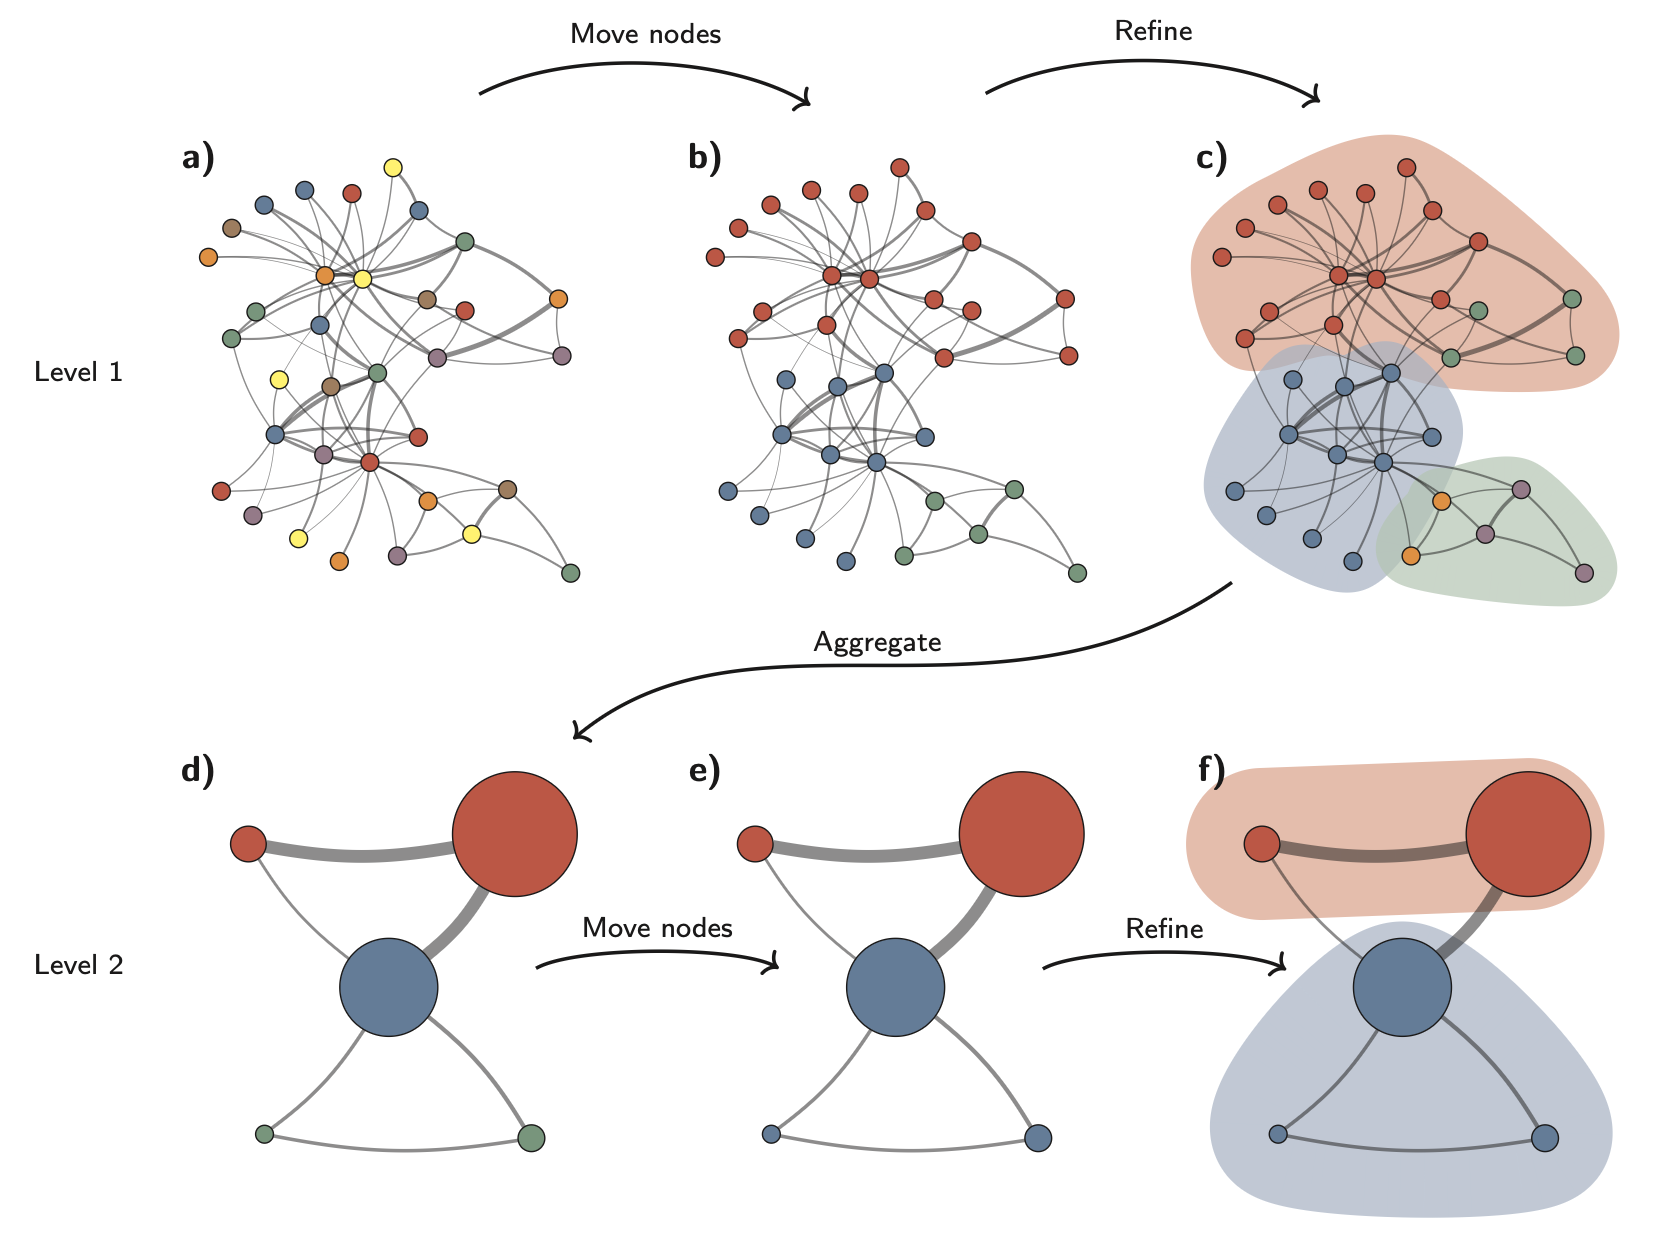
\includegraphics[width=0.9\textwidth]{img/Leiden_example.png}
    \caption{Illustration of the Leiden algorithm process. The algorithm starts from a singleton partition (a), moves nodes between communities (b), refines the partition (c), creates an aggregate network (d), moves nodes in the aggregate network (e), and refines again (f). These steps are repeated until no further improvements can be made. Figure adapted from \cite{leiden}.}
    \label{fig:leiden_algorithm}
\end{figure}

\subsection{Multi-view Anchor Graph-based Clustering (MVAGC)}
\label{subsec:MVAGC}

Multi-view Anchor Graph-based Clustering (MVAGC) is an advanced clustering technique designed to handle complex datasets represented by multiple feature sets or 'views'. 

The core idea of MVAGC is to leverage the complementary information present in these different views to obtain a more robust and meaningful clustering result than using any single view alone. Instead of working with the potentially very large full graph, MVAGC utilizes a smaller set of 'anchor points'. These anchors are selected representative points from the dataset (either strategically chosen or randomly sampled).

For each view of the data, MVAGC constructs a relationship matrix between data points and anchors. This relationship captures how strongly each data point connects to each anchor:

\begin{equation}
Z_{ij}^{(v)} = \frac{\text{similarity}(x_i, a_j)}{\sum_k \text{similarity}(x_i, a_k)}
\end{equation}

where $Z_{ij}^{(v)}$ indicates how strongly data point $i$ relates to anchor $j$ in view $v$, normalized to ensure the sum equals 1.

The key challenge is combining these different views into a unified representation. This can be expressed as finding a consensus matrix $Z^*$ that best approximates all individual views:

\begin{equation}
Z^* = \text{argmin} \sum_{v} \text{distance}(Z^{(v)}, Z^*)
\end{equation}

Once this consensus matrix is obtained, a similarity graph between all data points can be constructed:

\begin{equation}
S = Z^* \times Z^{*T}
\end{equation}

This similarity graph captures the relationships between all data points through their connections to the anchor points, making clustering more efficient by working with a smaller set of anchors instead of all possible pairwise connections.

\begin{algorithm}[H]
\caption{Multi-view Anchor Graph-based Clustering (MVAGC)}
\label{alg:mvagc}
\begin{algorithmic}[1]
\Require Data points $V = \{v_1, \dots, v_n\}$, Multiple view data representations $X^{(1)}, \dots, X^{(p)}$, Number of clusters $k$, Number of anchors $m$
\Ensure Cluster assignments for vertices $V$

\State Select $m$ anchor points $U = \{u_1, \dots, u_m\}$ from $V$ (e.g., using k-means or random sampling).
\For{each view $v = 1, \dots, p$}
    \State Construct view-specific anchor relationship matrix $Z^{(v)} \in \R^{n \times m}$. $Z_{ij}^{(v)}$ represents the similarity/connection between data point $v_i$ and anchor $u_j$ in view $v$.
\EndFor
\State Fuse the view-specific matrices $\{Z^{(1)}, \dots, Z^{(p)}\}$ into a unified representation. This often involves solving an optimization problem to find a consensus matrix $Z^*$ or graph structure that integrates information across views. 
    \Comment{E.g., Minimize $\sum_{v=1}^{p} \| Z^{(v)} - \text{f}(Z^*, \dots) \|_F^2 + \lambda \cdot \text{Regularization}(Z^*)$}
\State Perform clustering based on the fused representation $Z^*$.
    \If{$Z^*$ represents point-to-anchor assignments}
        \State Apply k-means or spectral clustering on the rows of $Z^*$ (representing points in the anchor space).
    \ElsIf{$Z^*$ is used to derive a consensus anchor graph $A_{\text{anchor}} \in \R^{m \times m}$}
        \State Apply spectral clustering on $A_{\text{anchor}}$ to cluster the anchors.
        \State Assign original points $v_i$ to the cluster of their nearest anchor based on $Z^*$.
    \EndIf
\State Assign final cluster labels $C_1, \dots, C_k$ to the original data points $V$.

\end{algorithmic}
\end{algorithm}

\section{Shortest Path Algorithms}
\label{se:ShortestPathAlgorithms}

Shortest path algorithms are fundamental for transportation network analysis, allowing us to determine the most efficient route between locations. In our work, we focused primarily on Dijkstra's algorithm due to its efficiency and suitability for transportation networks with non-negative edge weights.

\subsection{Dijkstra's Algorithm}
\label{subsec:DijkstrasAlgorithm}

Dijkstra's algorithm solves the single-source shortest path problem for a weighted graph with non-negative edge weights. Given a weighted graph $G = (V, E)$ with vertices $V$ and edges $E$, and a source vertex $s \in V$, Dijkstra's algorithm finds the shortest path from $s$ to every other vertex in the graph.

For a weighted graph $G = (V, E)$ with a weight function $w: E \rightarrow \mathbb{R}^+$ (assigning non-negative weights to edges), Dijkstra's algorithm maintains two primary values for each vertex $v \in V$: First, $\text{dist}[v]$ represents the currently known shortest distance from source $s$ to vertex $v$; Second, $\text{prev}[v]$ indicates the predecessor of $v$ in the shortest path from $s$ to $v$.

The algorithm initializes $\text{dist}[s] = 0$ and $\text{dist}[v] = \infty$ for all other vertices $v \in V \setminus \{s\}$. The iterative process then begins by selecting the unvisited vertex $u$ with the smallest distance value $\text{dist}[u]$. After marking $u$ as visited, the algorithm updates the distance values of all neighboring vertices $v$ according to the following formula:

\begin{equation}
\text{dist}[v] = \min(\text{dist}[v], \text{dist}[u] + w(u, v))
\end{equation}

where $w(u, v)$ is the weight of the edge from $u$ to $v$.

When a shorter path is discovered and the distance is updated, the predecessor is also updated:

\begin{equation}
\text{prev}[v] = u
\end{equation}

This equation updates the predecessor pointer when a shorter path is found. After Dijkstra's algorithm completes, these predecessor pointers can be used to reconstruct the actual shortest path from source to any destination vertex. The complete path from source $s$ to target vertex $t$ can be obtained by recursively following the predecessor pointers, starting from $t$ and working backward until reaching $s$:

\begin{equation}
\text{Path}(s, t) = 
\begin{cases}
\langle s \rangle & \text{if } s = t \\
\text{Path}(s, \text{prev}[t]) \cdot \langle t \rangle & \text{otherwise}
\end{cases}
\end{equation}

where $\cdot$ denotes path concatenation. This recursive definition builds the path by starting at the destination and tracing back through predecessors until reaching the source.

\begin{algorithm}[H]
\caption{Dijkstra's Shortest Path Algorithm}
\label{alg:dijkstra}
\begin{algorithmic}[1]
\Require Graph $G = (V, E)$, Source vertex $s \in V$, Weight function $w: E \rightarrow \mathbb{R}^+$
\Ensure Shortest path from $s$ to all vertices in $V$

\State Initialize $\text{dist}[s] \gets 0$ and $\text{dist}[v] \gets \infty$ for all $v \in V \setminus \{s\}$
\State Initialize $\text{prev}[v] \gets \text{null}$ for all $v \in V$
\State Initialize set of unvisited vertices $Q \gets V$

\While{$Q \neq \emptyset$}
    \State $u \gets \text{vertex in } Q \text{ with min } \text{dist}[u]$ \Comment{Extract min operation}
    \State Remove $u$ from $Q$
    
    \For{each neighbor $v$ of $u$ in $G$}
        \State $\text{alt} \gets \text{dist}[u] + w(u, v)$ \Comment{Distance through $u$ to $v$}
        \If{$\text{alt} < \text{dist}[v]$}
            \State $\text{dist}[v] \gets \text{alt}$ \Comment{Update distance}
            \State $\text{prev}[v] \gets u$ \Comment{Update predecessor}
        \EndIf
    \EndFor
\EndWhile

\State \Return $\text{dist}$ and $\text{prev}$ arrays
\end{algorithmic}
\end{algorithm}

\section{Outlier Detection}
\label{se:OutlierDetection}

Before analyzing network structures like communities or shortest paths, it is often crucial to identify and handle outliers in the data. Outliers, which are data points significantly different from the majority, can arise from various sources such as data entry errors, measurement inaccuracies, or genuinely unusual but valid observations. In the context of transportation networks represented as graphs, outliers might correspond to geographically isolated locations, incorrectly mapped points, or densely clustered points representing duplicates. Failing to address outliers can skew the results of subsequent analyses like clustering or pathfinding. Various methods exist for outlier detection in spatial or graph data.

\subsection{K-Nearest Neighbor (KNN) Outliers}
\label{subsec:KNNDistanceOutlier}

The K-Nearest Neighbor (KNN) distance-based outlier detection method identifies outliers by examining the local density of data points \cite{knn_outlier}. The core principle is that normal data points tend to have a similar density of neighbors, whereas outliers often reside in sparser regions (isolated points) or unusually dense regions (potential duplicates or overlapping points).

The algorithm calculates, for each data point $p$, the distance to its $k$-th nearest neighbor, denoted as $d_k(p)$, or alternatively, the average distance to its $k$ nearest neighbors. Points with significantly larger $d_k(p)$ values compared to the rest of the dataset are considered potential outliers, as they are relatively isolated. Conversely, points with unusually small distances (approaching zero) might indicate duplicate entries or points that are too close to be distinct locations in the context of the analysis.

To formally identify outliers, a threshold is typically established based on the distribution of these KNN distances. For instance, points whose KNN distance exceeds a certain number of standard deviations from the mean KNN distance across all points can be flagged as outliers. The choice of $k$ is a critical parameter, influencing the algorithm's sensitivity to local density variations. A smaller $k$ detects outliers based on very local neighborhoods, while a larger $k$ considers a broader context.

\begin{algorithm}[H]
\caption{KNN Distance-Based Outlier Detection}
\label{alg:knn_outlier}
\begin{algorithmic}[1]
\Require Dataset $D = \{p_1, \dots, p_n\}$, integer $k$, threshold $t$
\Ensure Set of outliers $O$

\State Initialize $O \gets \emptyset$
\State Initialize $knn\_distances \gets \emptyset$
\For{each point $p_i \in D$}
    \State Find the $k$ nearest neighbors $N_k(p_i)$ of $p_i$ in $D \setminus \{p_i\}$
    \State Calculate the average distance to the $k$ neighbors: $avg\_dist(p_i) = \frac{1}{k} \sum_{p_j \in N_k(p_i)} \text{distance}(p_i, p_j)$
    \Comment{Alternatively, use distance to $k$-th neighbor: $d_k(p_i) = \text{distance}(p_i, p_k)$, where $p_k$ is the $k$-th neighbor}
    \State Add $avg\_dist(p_i)$ to $knn\_distances$
\EndFor
\State Calculate mean $\mu$ and standard deviation $\sigma$ of values in $knn\_distances$
\For{each point $p_i \in D$}
    \If{$|avg\_dist(p_i) - \mu| > t \cdot \sigma$}
        \State Add $p_i$ to $O$
    \EndIf
\EndFor
\State \Return $O$
\end{algorithmic}
\end{algorithm}
